\documentclass[10pt,aspectratio=169]{beamer}

% --- Custom Colors ---
\definecolor{ulbblue}{RGB}{0, 51, 102}
\definecolor{ulbgold}{RGB}{204, 153, 0}
\definecolor{darkslate}{RGB}{30, 41, 59}
\definecolor{lightbg}{RGB}{248, 249, 250}
\definecolor{mathred}{RGB}{180, 30, 30}
\definecolor{mathgreen}{RGB}{20, 120, 40}

% --- Theme and Color Assignments ---
\usetheme{Madrid}
\usecolortheme{whale}
\setbeamertemplate{navigation symbols}{}
\setbeamertemplate{headline}{}

\setbeamercolor{palette primary}{bg=ulbblue,fg=white}
\setbeamercolor{palette secondary}{bg=ulbblue!85,fg=white}
\setbeamercolor{palette tertiary}{bg=ulbblue!70,fg=white}
\setbeamercolor{titlelike}{parent=palette primary}
\setbeamercolor{block title}{bg=ulbblue,fg=white}
\setbeamercolor{block body}{bg=lightbg,fg=darkslate}
\setbeamercolor{alertblock title}{bg=mathred,fg=white}
\setbeamercolor{alertblock body}{bg=lightbg,fg=darkslate}
\setbeamercolor{exampleblock title}{bg=mathgreen,fg=white}
\setbeamercolor{exampleblock body}{bg=lightbg,fg=darkslate}

% --- Packages ---
\usepackage[utf8]{inputenc}
\usepackage[T1]{fontenc}
\usepackage{amsmath,amssymb,amsfonts,mathtools}
\usepackage{booktabs}
\usepackage{siunitx}
\usepackage{tikz}
\usetikzlibrary{arrows.meta,positioning,calc}

% --- Custom Math Operators ---
\DeclareMathOperator{\FT}{\mathcal{F}}
\newcommand{\dd}{\mathrm{d}}
\newcommand{\jj}{\mathrm{j}}

\usepackage{mathtools}  
\mathtoolsset{showonlyrefs} % TO REMOVE QUEATION NUMBERING IF NOT CITED/REFERENCED

% --- Presentation Metadata ---
\title[Time Dispersion \& Frequency Selectivity]{Time Dispersion and Frequency Selectivity}
\subtitle{Derivations and Applied Case Study at 60 GHz - ELEC-H415 (Chapter 1)}
\author[Lucas Placentino]{Lucas Placentino}
\institute[EPB-ULB]{École Polytechnique de Bruxelles - Université Libre de Bruxelles}
\date{2026}

\begin{document}

% =============================================================================
% Slide 1: Title Slide
% =============================================================================
\begin{frame}
  \titlepage
\end{frame}

% =============================================================================
% Slide 2: Case Study Setup [~1.5 min]
% =============================================================================
\begin{frame}{Applied Case Study: Indoor 60 GHz Wireless Communication}
  \begin{columns}[T]
    \begin{column}{0.54\textwidth}
      \textbf{Indoor Measurement Setup (Course Fig.~1.2--1.3):}
      \begin{itemize}
        \item Carrier frequency: $f_c = \SI{60}{\giga\hertz}$ ($\lambda = c/f_c = \SI{5}{\milli\meter}$).
        \item Baseband bandwidth: $B = \SI{2.0}{\giga\hertz}$ ($f \in [-1, +1]\text{ GHz}$).
        \item Channel geometry:
        \begin{enumerate}
          \item \textbf{Direct Path (Path 1):} Distance $d_1 = \SI{3.0}{\meter}$.
          \item \textbf{Wall Reflected Path (Path 2):} Distance $d_2 = \SI{4.5}{\meter}$, reflection coefficient $\Gamma = -0.6 = 0.6 e^{\jj\pi}$.
        \end{enumerate}
      \end{itemize}
    \end{column}
    \begin{column}{0.44\textwidth}
      \begin{center}
        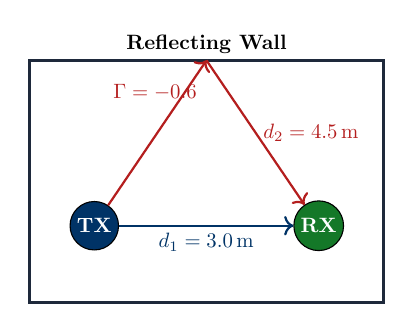
\begin{tikzpicture}[scale=0.75, every node/.style={transform shape}]
          \draw[very thick, darkslate] (-0.5,-0.5) rectangle (5.5,3.6);
          \node[above] at (2.5,3.6) {\textbf{Reflecting Wall}};
          
          \node[draw, fill=ulbblue, text=white, circle, inner sep=2pt] (TX) at (0.6,0.8) {\textbf{TX}};
          \node[draw, fill=mathgreen, text=white, circle, inner sep=2pt] (RX) at (4.4,0.8) {\textbf{RX}};
          
          % Direct Path
          \draw[thick, ulbblue, ->] (TX) -- node[midway, below] {$d_1 = \SI{3.0}{m}$} (RX);
          
          % Reflected Path
          \draw[thick, mathred, ->] (TX) -- (2.5,3.6);
          \draw[thick, mathred, ->] (2.5,3.6) -- node[midway, right] {$d_2 = \SI{4.5}{m}$} (RX);
          \node[above right, mathred] at (0.8,2.8) {$\Gamma = -0.6$};
        \end{tikzpicture}
      \end{center}
      \begin{alertblock}{Objective}
        Derive how multipath delays distort the transmitted spectrum $|H(f)|$ across the $\SI{2}{\giga\hertz}$ bandwidth from physical principles.
      \end{alertblock}
    \end{column}
  \end{columns}
\end{frame}

% =============================================================================
% Slide 3: Passband Wave Propagation [~1.5 min]
% =============================================================================
\begin{frame}{Step 1A: Passband Propagation for a Single Path}
  Let the transmitter emit an unmodulated carrier at frequency $f_c$:
  \begin{equation}
    x_{\mathrm{RF}}(t) = \cos(2\pi f_c t)
  \end{equation}

  Along physical path $n$, the wave propagates over distance $d_n$ with speed $c$:
  \begin{itemize}
    \item \textbf{Propagation Delay:} $\tau_n = d_n / c$.
    \item \textbf{Channel Attenuation:} $a_n \in \mathbb{R}^+$ %(free-space geometric divergence + reflection losses).
    \item \textbf{Phase Shift:} $\phi_n \in [0, 2\pi)$ %(material reflection phase, antenna effects).
    %\item \textbf{Boundary Phase Shift:} $\phi_n \in [0, 2\pi)$ %(material reflection phase, antenna effects).
  \end{itemize}

  \begin{block}{Received Passband Signal on Path $n$}
    \begin{align}
      y_{\mathrm{RF}, n}(t) &= a_n \cos\left( 2\pi f_c (t - \tau_n) + \phi_n \right) \nonumber \\
                            &= a_n \cos\left( 2\pi f_c t + (\phi_n - 2\pi f_c \tau_n) \right)
    \end{align}
  \end{block}
  The carrier undergoes a total phase rotation: $\theta_n = \phi_n - 2\pi f_c \tau_n$.
\end{frame}

% =============================================================================
% Slide 4: Baseband Conversion Derivation [~1.5 min]
% =============================================================================
\begin{frame}{Step 1B: Passband to Baseband}
  Using complex analytic signal representation:
  \begin{equation}
    y_{\mathrm{RF}, n}(t) = \operatorname{Re}\left\{ y_n(t) \, e^{\jj 2\pi f_c t} \right\}
  \end{equation}
  where $y_n(t) \in \mathbb{C}$ is the baseband representation of the received signal.

  \begin{align}
    y_{\mathrm{RF}, n}(t) &= a_n \cos\left( 2\pi f_c t + (\phi_n - 2\pi f_c \tau_n) \right) \nonumber \\
                          &= \operatorname{Re}\left\{ \left( a_n e^{\jj\phi_n} e^{-\jj 2\pi f_c \tau_n} \right) e^{\jj 2\pi f_c t} \right\}
  \end{align}

  \begin{block}{Complex Channel Amplitude $\alpha_n$}
    \begin{equation}
      \boxed{y_n(t) = a_n e^{\jj\phi_n} e^{-\jj 2\pi f_c \tau_n} \triangleq \alpha_n}
    \end{equation}
  \end{block}
  When the carrier is modulated by an arbitrary baseband signal $x(t)$:
  \begin{equation}
    x_{\mathrm{RF}}(t) = \operatorname{Re}\left\{ x(t) e^{\jj 2\pi f_c t} \right\} \implies \boxed{y_n(t) = \alpha_n \, x(t - \tau_n)}
  \end{equation}
\end{frame}

% =============================================================================
% Slide 5: Phase Sensitivity Analysis [~1.5 min]
% =============================================================================
\begin{frame}{Step 1C: Phase Sensitivity at 60 GHz vs. Sub-6 GHz}
  The carrier phase term is directly proportional to physical distance $d_n$:
  \begin{equation}
    \theta_n = -2\pi f_c \tau_n = -2\pi f_c \frac{d_n}{c} = -2\pi \frac{d_n}{\lambda_c}
  \end{equation}

  Taking the spatial derivative with respect to path length $d_n$:
  \begin{equation}
    \boxed{\frac{\partial \theta_n}{\partial d_n} = -\frac{2\pi}{\lambda_c} = -\frac{2\pi f_c}{c}}
  \end{equation}

  \begin{columns}[T]
    \begin{column}{0.48\textwidth}
      \begin{exampleblock}{Sub-6 GHz ($f_c = \SI{1}{\giga\hertz}$)}
        \begin{itemize}
          \item $\lambda_c = \SI{30}{\centi\meter}$.
          \item $\Delta d = \SI{15}{\centi\meter} \implies \Delta\theta = \pi$ (inversion).
          \item Large movements needed to alter $\alpha_n$.
        \end{itemize}
      \end{exampleblock}
    \end{column}

    \begin{column}{0.48\textwidth}
      \begin{alertblock}{5G mmWave ($f_c = \SI{60}{\giga\hertz}$)}
        \begin{itemize}
          \item $\lambda_c = \SI{5}{\milli\meter}$.
          \item $\Delta d = \SI{2.5}{\milli\meter} \implies \Delta\theta = \pi$ (inversion).
          \item \textbf{Small movements} completely randomize the complex amplitude phase.
        \end{itemize}
      \end{alertblock}
    \end{column}
  \end{columns}
\end{frame}

% =============================================================================
% Slide 6: Multipath Superposition & Impulse Response [~1.5 min]
% =============================================================================
\begin{frame}{Step 2: Multipath Superposition \& Impulse Response $h(\tau)$}
  In a real propagation channel, the received signal is the sum of $N$ distinct physical paths:
  \begin{equation}
    y(t) = \sum_{n=1}^{N} a_n e^{\jj\phi_n} e^{-\jj 2\pi f_c \tau_n} x(t - \tau_n) = \sum_{n=1}^{N} \alpha_n x(t - \tau_n)
  \end{equation}

  \begin{columns}[T]
    \begin{column}{0.50\textwidth}
      \textbf{Dirac Excitation $x(t) = \delta(t)$:}
      \begin{equation}
        y(t) = \sum_{n=1}^{N} \alpha_n \delta(t - \tau_n)
      \end{equation}
      \begin{block}{Baseband Channel Impulse Response}
        \begin{equation}
          \boxed{h(\tau) = \sum_{n=1}^{N} \alpha_n \delta(\tau - \tau_n)}
        \end{equation}
        where $\alpha_n = a_n e^{\jj\phi_n} e^{-\jj 2\pi f_c \tau_n}$.
      \end{block}
    \end{column}

    \begin{column}{0.48\textwidth}
      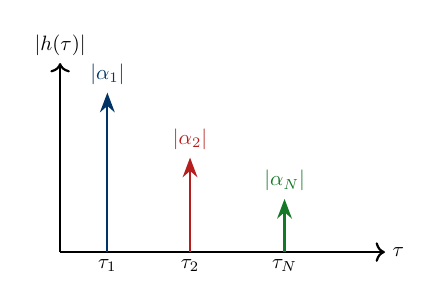
\begin{tikzpicture}[scale=0.75, every node/.style={transform shape}]
        \draw[->, thick] (0,0) -- (5.5,0) node[right] {$\tau$};
        \draw[->, thick] (0,0) -- (0,3.2) node[above] {$|h(\tau)|$};
        
        \draw[thick, ulbblue, -{Stealth[length=2.5mm]}] (0.8,0) -- (0.8,2.7) node[above] {$|\alpha_1|$};
        \draw[thick, mathred, -{Stealth[length=2.5mm]}] (2.2,0) -- (2.2,1.6) node[above] {$|\alpha_2|$};
        \draw[thick, mathgreen, -{Stealth[length=2.5mm]}] (3.8,0) -- (3.8,0.9) node[above] {$|\alpha_N|$};
        
        \node[below] at (0.8,0) {$\tau_1$};
        \node[below] at (2.2,0) {$\tau_2$};
        \node[below] at (3.8,0) {$\tau_N$};
      \end{tikzpicture}
      \begin{itemize}
        \item $h(\tau)$ is a sum of Dirac distributions.
        \item Fully characterizes channel physics in delay domain $\tau$.
      \end{itemize}
    \end{column}
  \end{columns}
\end{frame}

% =============================================================================
% Slide 7: Input-Output Convolution [~1.5 min]
% =============================================================================
\begin{frame}{Step 3: Input-Output Relationship as a Convolution}
  Using the "sifting" property of Dirac distributions:
  \begin{equation}
    x(t - \tau_n) = \int_{0}^{\infty} \delta(\tau - \tau_n) x(t - \tau) \,\dd\tau
  \end{equation}
  Substituting into $y(t) = \sum_{n=1}^N \alpha_n x(t - \tau_n)$:
  \begin{equation}
    y(t) = \sum_{n=1}^{N} \alpha_n \int_{0}^{\infty} \delta(\tau - \tau_n) x(t - \tau) \,\dd\tau = \int_{0}^{\infty} \underbrace{\left[ \sum_{n=1}^{N} \alpha_n \delta(\tau - \tau_n) \right]}_{= h(\tau)} x(t - \tau) \,\dd\tau
  \end{equation}

  \begin{block}{Convolution Product}
    \begin{equation}
      \boxed{y(t) = \int_{0}^{\infty} h(\tau) x(t - \tau) \,\dd\tau = (h * x)(t)}
    \end{equation}
  \end{block}
  \textbf{Physical Interpretation of Time Dispersion:}
  When the transmitter sends one single impulse, the receiver perceives multiple delayed copies spread over time.
\end{frame}

% =============================================================================
% Slide 8: Continuous Fourier Derivation [~2 min]
% =============================================================================
\begin{frame}{Step 4: Derivation of the Channel Transfer Function $H(f)$}
\small
  We compute the Fourier transform of $y(t) = \int_{-\infty}^{\infty} h(\tau) x(t - \tau) \,\dd\tau$ with respect to time $t$:
  \begin{equation}
    Y(f) = \int_{-\infty}^{\infty} y(t) e^{-\jj 2\pi f t} \,\dd t = \int_{-\infty}^{\infty} \left[ \int_{-\infty}^{\infty} h(\tau) x(t - \tau) \,\dd\tau \right] e^{-\jj 2\pi f t} \,\dd t
  \end{equation}
  Interchanging integrals via Fubini's theorem:
  \begin{equation}
    Y(f) = \int_{-\infty}^{\infty} h(\tau) \left[ \int_{-\infty}^{\infty} x(t - \tau) e^{-\jj 2\pi f t} \,\dd t \right] \dd\tau
  \end{equation}
  Applying substitution $u = t - \tau \implies t = u + \tau$ and $\dd t = \dd u$:
  \begin{align}
    Y(f) &= \int_{-\infty}^{\infty} h(\tau) \left[ \int_{-\infty}^{\infty} x(u) e^{-\jj 2\pi f (u + \tau)} \,\dd u \right] \dd\tau \nonumber \\
         &= \left( \int_{-\infty}^{\infty} h(\tau) e^{-\jj 2\pi f \tau} \,\dd\tau \right) \underbrace{\left( \int_{-\infty}^{\infty} x(u) e^{-\jj 2\pi f u} \,\dd u \right)}_{= X(f)}
  \end{align}
  \vspace{-1em}
  \begin{block}{Baseband Transfer Function}
    \begin{equation}
      \boxed{H(f) \triangleq \int_{-\infty}^{\infty} h(\tau) e^{-\jj 2\pi f \tau} \,\dd\tau} \implies \boxed{Y(f) = H(f) X(f)}
    \end{equation}
  \end{block}
\end{frame}

% =============================================================================
% Slide 9: Discrete Multipath Transfer Function [~1.5 min]
% =============================================================================
\begin{frame}{Step 5: Transfer Function for Discrete Multipath Components}
\small
  Injecting $h(\tau) = \sum_{n=1}^N \alpha_n \delta(\tau - \tau_n)$ into the Fourier transform definition:
  \begin{align}
    H(f) &= \int_{-\infty}^{\infty} \left[ \sum_{n=1}^{N} \alpha_n \delta(\tau - \tau_n) \right] e^{-\jj 2\pi f \tau} \,\dd\tau \nonumber \\
         &= \sum_{n=1}^{N} \alpha_n \int_{-\infty}^{\infty} \delta(\tau - \tau_n) e^{-\jj 2\pi f \tau} \,\dd\tau
  \end{align}
  Applying the Dirac integral:
  \begin{equation}
    \boxed{H(f) = \sum_{n=1}^{N} \alpha_n e^{-\jj 2\pi f \tau_n} = \sum_{n=1}^{N} a_n e^{\jj\phi_n} e^{-\jj 2\pi f_c \tau_n} e^{-\jj 2\pi f \tau_n}}
  \end{equation}
\vspace{-1em}
  \begin{alertblock}{Total Path Phase}
    \begin{equation}
      H(f) = \sum_{n=1}^{N} a_n e^{\jj\phi_n} e^{-\jj 2\pi (f_c + f)\tau_n}
    \end{equation}
    \vspace{-1em}
    \begin{itemize}
      \item $f_c$ sets the microscopic path phase ($\SI{60}{\giga\hertz}$ carrier).
      \item $f$ sets the frequency-dependent phase slope across the baseband spectrum ($\pm \SI{1}{\giga\hertz}$).
    \end{itemize}
  \end{alertblock}
\end{frame}

% =============================================================================
% Slide 10: Non-Selective vs Selective Regimes [~1.5 min]
% =============================================================================
\begin{frame}{Step 6: Mathematical Proof of Frequency Selectivity}
\small
  \begin{columns}[T]
    \begin{column}{0.48\textwidth}
      \begin{exampleblock}{Case 1: No Time Dispersion ($\tau_n = \tau_1, \forall n$)}
        \begin{equation}
          H(f) = e^{-\jj 2\pi f \tau_1} \sum_{n=1}^N \alpha_n
        \end{equation}
        Computing the magnitude:
        \begin{equation}
          |H(f)| = \left| e^{-\jj 2\pi f \tau_1} \right| \cdot \left| \sum_{n=1}^N \alpha_n \right| = \left| \sum_{n=1}^N \alpha_n \right|
        \end{equation}
        \begin{itemize}
          \item $|H(f)|$ is \textbf{constant over bandwidth $B$}.
          \item Signal spectrum is not distorted.
          \item \textbf{Non-frequency-selective (Flat channel)}.
        \end{itemize}
      \end{exampleblock}
    \end{column}

    \begin{column}{0.48\textwidth}
      \begin{alertblock}{Case 2: Arbitrary Delays ($\exists \tau_n \neq \tau_m$)}
        \begin{equation}
          |H(f)| = \left| \sum_{n=1}^{N} \alpha_n e^{-\jj 2\pi f \tau_n} \right|
        \end{equation}
        \begin{itemize}
          \item $|H(f)|$ \textbf{varies with baseband frequency $f$}.
          \item Multipaths interfere constructively at some frequencies and destructively at others.
          \item \textbf{Frequency-selective channel}.
        \end{itemize}
      \end{alertblock}
    \end{column}
  \end{columns}

  \begin{block}{Fundamental Principle}
    \centering
    \textbf{Time dispersion during propagation $\iff$ Frequency selectivity across bandwidth.}
  \end{block}
\end{frame}

% =============================================================================
% Slide 11: Physical Interference Mechanism [~1.5 min]
% =============================================================================
\begin{frame}{Step 7: The Physical Interference Process}
  Every copy $n$ arrives with baseband phase $-2\pi f \tau_n$.

  \begin{block}{Phase Difference Between Two Paths $n$ and $m$}
    \begin{equation}
      \Delta\Phi_{nm}(f) = -2\pi f (\tau_n - \tau_m)
    \end{equation}
  \end{block}

  \begin{itemize}
    \setlength{\itemsep}{0.25cm}
    \item \textbf{Frequency Dependence:}
    \begin{itemize}
      \item When $\Delta\Phi_{nm}(f) = 2k\pi$: constructive interference $\implies |H(f)|$ reaches a local maximum.
      \item When $\Delta\Phi_{nm}(f) = (2k+1)\pi$: destructive interference $\implies |H(f)|$ reaches a local minimum.
    \end{itemize}
    \item \textbf{Delay Difference Dependence:} The speed of phase rotation with respect to $f$ is:
    \begin{equation}
      \left| \frac{\dd \Delta\Phi_{nm}}{\dd f} \right| = 2\pi |\tau_n - \tau_m|
    \end{equation}
    \item \textbf{Physical Consequence:} The larger the delay spread $|\tau_n - \tau_m|$, the faster the phase changes with $f$, making \textbf{frequency selectivity more severe}.
  \end{itemize}
\end{frame}

% =============================================================================
% Slide 12: Quantitative Case Study - Path Parameters [~1.5 min]
% =============================================================================
\begin{frame}{Step 8A: 60 GHz Case Study, Exact Path Calculation}
  \begin{columns}[T]
    \begin{column}{0.48\textwidth}
      \textbf{1. Direct Path ($n=1$):}
      \begin{itemize}
        \item Delay:
        \begin{equation}
          \tau_1 = \frac{d_1}{c} = \frac{\SI{3.0}{\meter}}{3 \times 10^8\text{ m/s}} = \mathbf{10.0\text{ \textbf{ns}}}
        \end{equation}
        \item Free-space normalization: $a_1 = 1.0$, $\phi_1 = 0$.
        \item Complex gain:
        \begin{align}
          \alpha_1 &= 1.0 \cdot e^{-\jj 2\pi (60 \times 10^9)(10 \times 10^{-9})} \nonumber \\
                   &= 1.0 \cdot e^{-\jj 1200\pi} = \mathbf{1.0}
        \end{align}
      \end{itemize}
    \end{column}

    \begin{column}{0.48\textwidth}
      \textbf{2. Reflected Path ($n=2$):}
      \begin{itemize}
        \item Delay:
        \begin{equation}
          \tau_2 = \frac{d_2}{c} = \frac{\SI{4.5}{\meter}}{3 \times 10^8\text{ m/s}} = \mathbf{15.0\text{ \textbf{ns}}}
        \end{equation}
        \item Amplitude: $a_2 = |\Gamma| \frac{d_1}{d_2} = 0.6 \times \frac{3.0}{4.5} = \mathbf{0.4}$.
        \item Reflection phase: $\phi_2 = \pi$ (from $\Gamma = -0.6$).
        \item Complex gain:
        \begin{align}
          \alpha_2 &= 0.4 \, e^{\jj\pi} \, e^{-\jj 2\pi (60 \times 10^9)(15 \times 10^{-9})} \nonumber \\
                   &= 0.4 \, e^{\jj\pi} \, e^{-\jj 1800\pi} = \mathbf{-0.4}
        \end{align}
      \end{itemize}
    \end{column}
  \end{columns}

  \begin{exampleblock}{Delay Spread}
    \begin{equation}
      \Delta\tau = \tau_2 - \tau_1 = \SI{15.0}{\nano\second} - \SI{10.0}{\nano\second} = \mathbf{5.0\text{ \textbf{ns}}}
    \end{equation}
  \end{exampleblock}
\end{frame}

% =============================================================================
% Slide 13: Quantitative Case Study - Transfer Function [~1.5 min]
% =============================================================================
\begin{frame}{Step 8B: 60 GHz Case Study, Evaluating $|H(f)|$}
  The channel transfer function is:
  \begin{align}
    H(f) &= \alpha_1 e^{-\jj 2\pi f \tau_1} + \alpha_2 e^{-\jj 2\pi f \tau_2} \nonumber \\
         &= 1.0 \, e^{-\jj 2\pi f (10 \times 10^{-9})} - 0.4 \, e^{-\jj 2\pi f (15 \times 10^{-9})} \nonumber \\
         &= e^{-\jj 2\pi f \tau_1} \left( 1.0 - 0.4 \, e^{-\jj 2\pi f \Delta\tau} \right) \quad (\Delta\tau = \SI{5.0}{\nano\second})
  \end{align}

  \begin{columns}[T]
    \begin{column}{0.48\textwidth}
      \textbf{Magnitude Extrema:}
      \begin{itemize}
        \item \textbf{Constructive ($e^{-\jj 2\pi f \Delta\tau} = -1$):}
        \begin{equation}
          |H|_{\max} = 1.0 + 0.4 = 1.4 \implies \mathbf{+2.92\text{ \textbf{dB}}}
        \end{equation}
        \item \textbf{Destructive ($e^{-\jj 2\pi f \Delta\tau} = +1$):}
        \begin{equation}
          |H|_{\min} = 1.0 - 0.4 = 0.6 \implies \mathbf{-4.44\text{ \textbf{dB}}}
        \end{equation}
      \end{itemize}
    \end{column}

    \begin{column}{0.48\textwidth}
      \begin{alertblock}{Spectral Fading}
      \small
        \begin{itemize}
          \item Total variation across band:
          \begin{equation*}
            \Delta|H| = 2.92 - (-4.44) = \mathbf{7.36\text{ \textbf{dB}}}
          \end{equation*}
          \item Ripple frequency period:
          \begin{equation}
            \Delta f_{\mathrm{period}} = \frac{1}{\Delta\tau} = \frac{1}{\SI{5.0}{\nano\second}} = \mathbf{200\text{ \textbf{MHz}}}
          \end{equation}
          \item Over $B = \SI{2}{\giga\hertz}$, the transfer function executes $\frac{\SI{2000}{\mega\hertz}}{\SI{200}{\mega\hertz}} = \mathbf{10\text{ \textbf{fading cycles}}}$.
        \end{itemize}
      \end{alertblock}
    \end{column}
  \end{columns}
\end{frame}

% =============================================================================
% Slide 14: Course Experimental Data Analysis [~1.5 min]
% =============================================================================
\begin{frame}{Step 9: Comparison with Experimental Data}
\footnotesize
  \begin{columns}[T]
    \begin{column}{0.48\textwidth}
    \vspace{-1.8em}
    \begin{figure}
        \centering
        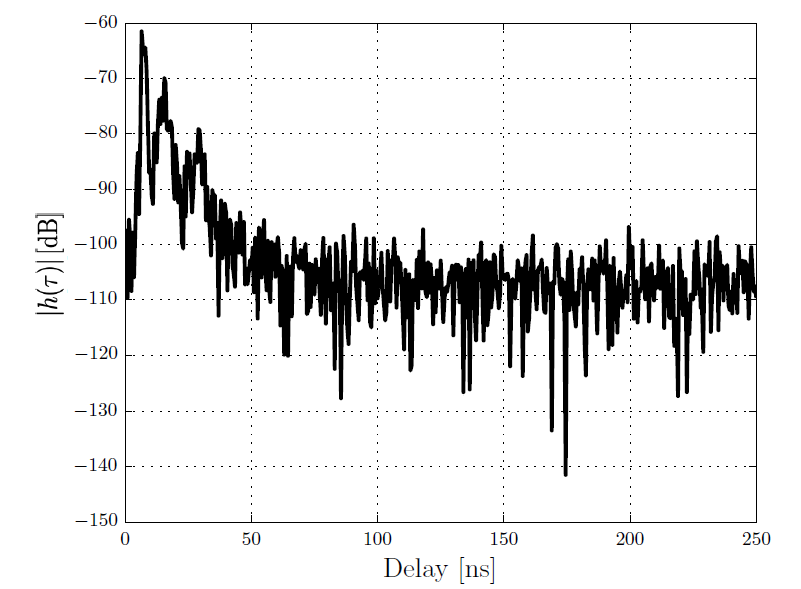
\includegraphics[width=0.7\linewidth]{delay-domain-time-dispersion-graph.png}
    \end{figure}
    \vspace{-1.6em}
      \begin{block}{\small Delay Domain: Figure 1.2 in Course}
        \centering
        \textbf{Experimental $|h(\tau)|$ (60 GHz, 2 GHz BW)}
        \begin{itemize}
          \item Measured via inverse Fourier transform over $\SI{2}{\giga\hertz}$ bandwidth.
          \item Shows direct path at $\tau \approx 0$ followed by dense multipath trail extending to $\SI{200}{\nano\second}$.
          \item Noise floor visible at $\approx \SI{-110}{\decibel}$.
        \end{itemize}
      \end{block}
    \end{column}

    \begin{column}{0.48\textwidth}
    \vspace{-1.8em}
    \begin{figure}
        \centering
        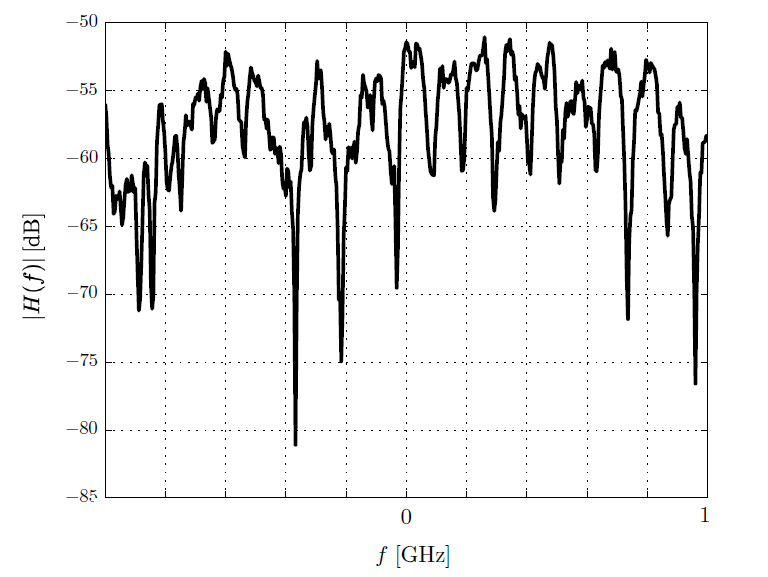
\includegraphics[width=0.7\linewidth]{frequency-selectivity-graph.png}
    \end{figure}
    \vspace{-1.6em}
      \begin{block}{\small Frequency Domain: Figure 1.3 in Course}
        \centering
        \textbf{Experimental $|H(f)|$ (60 GHz, 2 GHz BW)}
        \begin{itemize}
          \item Plotted across baseband frequency $f \in [-1, 1]\text{ GHz}$.
          \item Displays severe, rapid fluctuations ranging from $\SI{-52}{\decibel}$ down to $\SI{-80}{\decibel}$.
          \item Directly confirms destructive multi-ray cancellation across spectrum.
        \end{itemize}
      \end{block}
    \end{column}
  \end{columns}

  % \begin{alertblock}{\small Physical Conclusion}
  %   The rich multipath tail in Figure 1.2 creates the high-frequency spectral fluctuations in Figure 1.3 through the Fourier integral transform $H(f) = \FT_\tau\{h(\tau)\}$.
  % \end{alertblock}
\end{frame}

% =============================================================================
% Slide 15: Time-Variant Channels & Quasi-Static Limit [~1.5 min]
% =============================================================================
\begin{frame}{Step 10: Time-Variant Channels \& Quasi-Static Approximation}
  When transmitter, receiver, or obstacles move, amplitudes and phases vary over clock-time $t$:
  \begin{equation}
    h(\tau, t) = \sum_{n=1}^{N} a_n(t) e^{\jj\phi_n(t)} e^{-\jj 2\pi f_c \tau_n} \delta(\tau - \tau_n) = \sum_{n=1}^{N} \alpha_n(t) \delta(\tau - \tau_n)
  \end{equation}
  The general input-output relation becomes:
  \begin{equation}
    y(t) = \int_{0}^{\infty} h(\tau, t) x(t - \tau) \,\dd\tau \quad \text{(no longer a convolution product)}
  \end{equation}

  \begin{columns}[T]
    \begin{column}{0.50\textwidth}
      \textbf{Time-Variant Transfer Function:}
      \begin{equation}
        H(f, t) = \int_{-\infty}^{\infty} h(\tau, t) e^{-\jj 2\pi f \tau} \,\dd\tau
      \end{equation}
      Note: $Y(f) \neq H(f, t) X(f)$ in general.
    \end{column}
    \begin{column}{0.48\textwidth}
      \begin{block}{Quasi-Static Approximation}
        The channel is assumed \textbf{time-invariant during the transmission of each block of symbols}.
        \begin{itemize}
          \item $\tau$ (delay): fast multipath propagation ($\sim \si{\nano\second}$).
          \item $t$ (clock time): slow macroscopic motion ($\sim \si{\milli\second}$).
        \end{itemize}
      \end{block}
    \end{column}
  \end{columns}
\end{frame}

% =============================================================================
% Slide 16: Engineering Impact & OFDM Solution [~1.5 min]
% =============================================================================
\begin{frame}{Step 11: Engineering Impact \& Multi-Carrier Mitigation}
  \begin{columns}[T]
    \begin{column}{0.48\textwidth}
      \begin{alertblock}{The Problem: Waveform Distortion}
        \begin{itemize}
          \item Because $|H(f)|$ is not constant across bandwidth $B$, each spectral component $X(f)$ undergoes different complex scaling.
          \item In the time domain, this causes severe \textbf{Inter-Symbol Interference (ISI)}.
          \item Single-carrier systems require complex time-domain equalizers.
        \end{itemize}
      \end{alertblock}
    \end{column}

    \begin{column}{0.48\textwidth}
      \begin{exampleblock}{Modern Solution: Multi-Carrier (OFDM)}
        \begin{itemize}
          \item In modern standards (5G NR, Wi-Fi 6/7), the wideband bandwidth $B$ is divided into many narrow orthogonal subcarriers.
          \item Across each narrow subcarrier bandwidth, $|H(f)|$ is approximately constant.
          \item \textbf{Result:} Converts a wideband frequency-selective channel into narrowband flat-fading subchannels.
        \end{itemize}
        \textit{$\Rightarrow$ Covered in detail in Modulation and Coding course.}
      \end{exampleblock}
    \end{column}
  \end{columns}
\end{frame}

% =============================================================================
% Slide 17: Summary & Conclusion [~1 min]
% =============================================================================
\begin{frame}{Summary: Complete Logical Chain of Derivations}
  \begin{enumerate}
    \setlength{\itemsep}{0.22cm}
    \item \textbf{Baseband Conversion:} Path delay $\tau_n$ and carrier $f_c$ define the complex amplitude $\alpha_n = a_n e^{\jj\phi_n} e^{-\jj 2\pi f_c \tau_n}$, sensitive to millimeter movmeents at $\SI{60}{\giga\hertz}$.
    \item \textbf{Impulse Response:} Multipath superposition creates time dispersion: $h(\tau) = \sum_{n=1}^N \alpha_n \delta(\tau - \tau_n)$, yielding convolution $y(t) = (h*x)(t)$.
    \item \textbf{Fourier Duality:} Applying the Fourier transform to $y(t)$ proves $Y(f) = H(f)X(f)$ with $H(f) = \sum_{n=1}^N \alpha_n e^{-\jj 2\pi f \tau_n}$.
    \item \textbf{Selectivity Proof:}
    \begin{itemize}
      \item $\tau_n = \tau_1 \implies |H(f)| = \text{constant}$ (Flat channel).
      \item $\exists \tau_n \neq \tau_m \implies |H(f)|$ fluctuates with $f$ (Frequency-selective channel).
    \end{itemize}
    \item \textbf{Interference Physics:} Phase difference $\Delta\Phi(f) = -2\pi f (\tau_n - \tau_m)$ rotates across bandwidth, creating fading ripples with period $\Delta f = 1/\Delta\tau$.
  \end{enumerate}
\end{frame}

\end{document}